%%%%%%%%%%%%%%%%%%%%%%%%%%%%%%%%%%%%%%%%%
% Avi's Project Proposal
%
% Summer Research Project 
%
%%%%%%%%%%%%%%%%%%%%%%%%%%%%%%%%%%%%%%%%%

%----------------------------------------------------------------------------------------
%	PACKAGES AND DOCUMENT CONFIGURATIONS
%----------------------------------------------------------------------------------------

\documentclass{article}

\usepackage[version=3]{mhchem} % Package for chemical equation typesetting
\usepackage{siunitx} % Provides the \SI{}{} and \si{} command for typesetting SI units
\usepackage{graphicx} % Required for the inclusion of images
\usepackage{natbib} % Required to change bibliography style to APA
\usepackage{amsmath} % Required for some math elements 
\usepackage{gensymb}

\setlength\parindent{0pt} % Removes all indentation from paragraphs

\renewcommand{\labelenumi}{\alph{enumi}.} % Make numbering in the enumerate environment by letter rather than number (e.g. section 6)

%\usepackage{times} % Uncomment to use the Times New Roman font


%Code packages

\usepackage[utf8]{inputenc}
\usepackage{listings}
\usepackage{color}
% Code packages end


%----------------------------------------------------------------------------------------
%	DOCUMENT INFORMATION
%----------------------------------------------------------------------------------------

\title{Project Plan} % Title
			 
\author{Avi \textsc{Vajpeyi}} % Author name

\date{\today} % Date for the report

\begin{document}

\maketitle % Insert the title, author and date


%have an understanding of what you will do and why the work is necessary or desirable
%It outlines the approach you will take to carry out your task
%It provides a schedule or timeline for accomplishing the individual steps and overall goals of your project
%It encourages your mentor and his or her staff to make the arrangements necessary to accommodate you and your needs before your arrival




 \begin{abstract}
On September 14th, 2016, the Advanced Interferometer Gravitational-Wave Observatories detected the first gravitational wave \cite{DetectionPaper}. The detected wave had a very large Signal to Noise Ratio value, which made it stand out from the rest of the candidate events. This paper investigates an alternative detection statistic, involving the `Bayes Factor'. This detection statistic might prove to be more robust than SNR, as it may be able to better discern between strains due to gravitational waves, and strains due to noise. 
\end{abstract}

%----------------------------------------------------------------------------------------
%	SECTION 1
%----------------------------------------------------------------------------------------

\section{Introduction}

% How Ligo detects signals
 \indent The completion of the two Advanced Laser Interferometer Gravitational-Wave Observatories has led to the discovery of a gravitational-wave signal \cite{DetectionPaper}.Each of the advanced LIGO observatories uses a modified Michaelson Interferometer that measures the difference in the length of the orthogonal arms of the observatory, to detect the presence of a gravitational wave. On passing, a gravitational wave alters the difference between the arm lengths which helps determine the gravitational-wave strain amplitude. \\
  
  % how signal is found in data
  \indent To determine if a signal recorded by LIGO stores gravitational wave information, the signal is processed with two search techniques. The first search looks for generic transient waveforms in the signal. The second search is a match filtered search which compares the signal with templates of waveforms generated by general relativity.\\
  
  
  % Discussion on how background noise is removed with time shifts, and how data is ranked 
  \indent Both the search processes are made challenging due to the background noise present in the data, which can cause strains in the instrument similar to strains from gravitational waves. This background noise can be due defects in a mirror, the uncertainty in the number of photons traveling in a the laser beam (shot noise), seismic activity, or even thermal noise generated by the Brownian motion of electrons inside circuits. To discount strains due to this background noise from being considered as strains due to gravitational waves, the signal data from one LIGO observatory is compared with another LIGO observatory's data. To compare the signals, one of the them must be time shifted so that it matches the other signal's time period. After making the necessary time shift, events present in one signal but not the other signal become apparent. If the strain is not present in both signals, the strain must be due to noise present in one of the detectors, as a gravitational wave would be observed in both detectors. Hence, all the strains that cannot be correlated with a data set taken from another observatory are discounted as strains due to noise. This process cuts a majority of the strains that may have been present due to noise. We attempt discounting any remaining noise-strains by implementing a detection statistic, which ranks the strains according to the likelihood of the strain being due to a gravitational wave.\\
  
    % Talk about Time-frequency morphology classes, and how certain classes can be discounted? That is more specific to Generic...
  
  % SNR as a detection statistic 
  The detection statistic currently being used to rank the strains according to the probability of it being due to a gravitational wave, is the signal-to-noise ratio (SNR) detection technique. This method compares the power of the strain signal to the power of the remaining noise at a given point. Although the power of the noise is difficult to calculate, we know that this ranking process can make some gravitational wave strains stand out, as seen from the Fig~\ref{Fig:Detection}.  However, we believe that this method lacks the sensitivity to detect some gravitational waves, that might not have as high SNR  values as the strain of GW150914's did. Hence we would like to investigate an alternate detection statistic. Specifically, one which uses the Bayes Factor to rank strains. This detection statistic might help increase the detection rate of gravitational waves by a factor of 10.  
   
\begin{figure}[h]
	\caption{Search results of the generic transit search in which the first gravitational wave signal, marked GW150914, was detected. The wave strain of GW150914 stands out as the strongest strain in the entire search. Figure taken from \cite{DetectionPaper}}
	\centering
	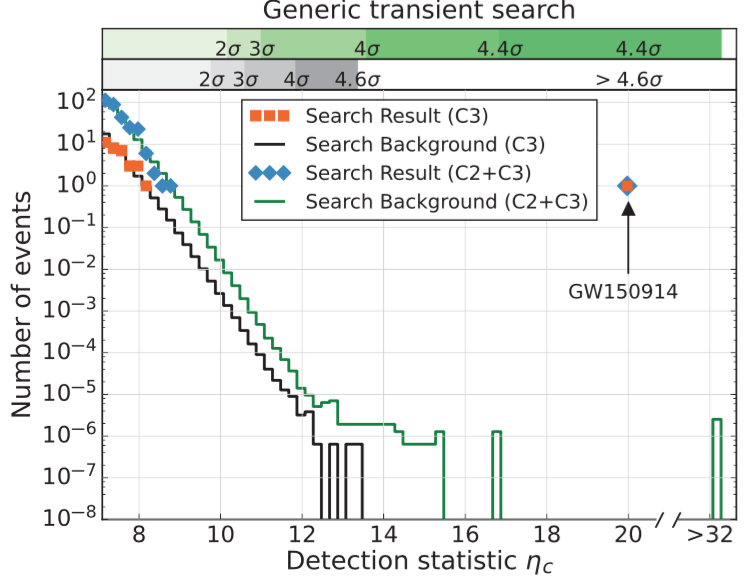
\includegraphics[width=0.5\textwidth]{DetectionInGenericTransientSearch} \label{Fig:Detection}
\end{figure}

 
 %----------------------------------------------------------------------------------------
 %	SECTION 2
 %----------------------------------------------------------------------------------------
 
 
 \section{Objectives}
 
 We have seen that using SNR for detection has been successful (as the gravitational wave GW150914 was detected with it) \cite{DetectionPaper}. However, we would like to investigate a more robust detection statistic, using the Bayes Factor. This detection statistic would involve comparing the probability that the signal data contains a strain due to gravitational waves, to the probability that the signal does not contain a strain due to a gravitational wave.\\
 
 This process may help highlight the strains due to gravitational waves against strains due to noise, and raise the number of gravitational wave detections. With more detections, we could have more data on the masses and spins of black holes in our universe. By combining these results of the data on black holes, we would be able to gain an estimate of the population of black holes in our universe. 
 %----------------------------------------------------------------------------------------
 %	SECTION 3
 %----------------------------------------------------------------------------------------
 
 
 \section{Approach}
 We will begin by creating a detection statistic procedure for gravitational waves using Bayesian analysis. We will then analyse the performance of the procedure by trying to detect injected gravitational waves strains (gravitation wave strains that are manually inserted into the signal data) amongst several other candidate events. If the procedure can detect the gravitational wave strains amongst the various other candidate strains due to noise, we will move onto studying how sensitive this new detection statistic is. To test its sensitivity, we will try to determine how low the signal to noise ratio must be before the procedure fails to detect the injected gravitational wave.
 
 %----------------------------------------------------------------------------------------
 %	SECTION 4
 %----------------------------------------------------------------------------------------
 
 
 \section{Project Schedule}
 
 %----------------------------------------------------------------------------------------
 %	REFERENCES
 %----------------------------------------------------------------------------------------
 
---------------------------------------------------------------------
 
 \bibliographystyle{plain}		% Using this bibliography style will ignore the annotations.
 
 \bibliography{ProjectProposalRefrences}
 
%----------------------------------------------------------------------------------------


\end{document}